\chapter{LITERATURE SURVEY	}
\hspace*{0.3in}This section consolidates major research contributions in the intersection of Quantum Computing (QC) and Artificial Intelligence (AI), referred to collectively as Quantum Artificial Intelligence (QAI). The works are grouped thematically to highlight foundations, system design strategies, natural language applications, real-world domains, industrial adoption, error correction efforts, and emerging trends.
\section{Quantum AI Foundations And Reviews}
\hspace*{0.3in}Recent surveys highlight how QAI is maturing into a distinct research field. The systematic literature review by Alzubi et al. (2025) synthesizes features and application domains where AI complements QC, ranging from calibration and simulation to optimization tasks [1]. Similarly, a review published in Path of Science (2025) emphasizes algorithmic advances in Quantum Support Vector Machines (QSVM), Quantum Neural Networks (QNN), and Quantum Reinforcement Learning (QRL), positioning them as building blocks of scalable QAI [2]. A broader comprehensive review (2025) situates QML within hybrid computational paradigms, describing transitions from quantum-enhanced classical models to fully native quantum approaches, while addressing challenges of scalability and hybrid integration [3].

\section{AI-Enhanced Quantum System Design And Error Correction}
\hspace*{0.3in}AI has been instrumental in refining quantum hardware control. A study on automatic re-calibration using reinforcement learning demonstrated model-free loops for maintaining stable device performance under drift conditions [4]. Extending this approach, deep reinforcement learning strategies for noise-adaptive qubit routing achieved reductions of up to 37.3\%
 in additional gates and increased success probabilities by 26.8\%
  on noisy devices [5]. Perhaps most notably, Google’s “Willow” processor (2025) introduced a 105-qubit platform that achieved error correction below the surface-code threshold, marking a breakthrough in exponential error suppression and demonstrating the synergy of AI-guided calibration with advanced hardware [6].
\section{Quantum Natural Language Processing (QNLP)}
\hspace*{0.3in}Language processing stands out as a complex yet promising domain. A 2024 survey on QNLP outlines how embeddings, sequential modeling, and attention can be transposed into quantum frameworks, thereby unlocking new pathways for semantic representation [7]. Building on this, the 2025 study on QNLP applications explores distributional compositional categorical models within quantum contexts, offering concrete examples where quantum systems outperform or augment classical NLP in handling ambiguity and compositionality [8].
\begin{figure}[htbp]
	\centering
	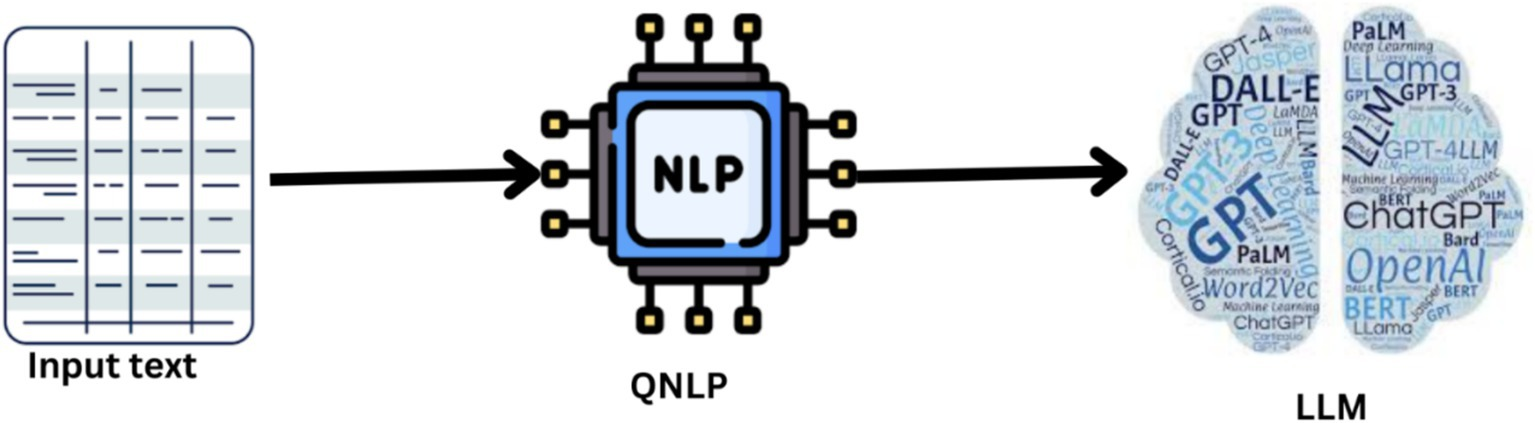
\includegraphics[width=1\linewidth]{qnlp.png}
	\caption{QLM model}
	\label{fig:enter-label}
\end{figure}
\section{Real-World Applications (Drug Discovery, Finance, Healthcare)}
\hspace*{0.3in}Translational impact is increasingly visible across scientific and industrial domains. For example, a study on QML-based electrokinetic mining illustrates how nanoparticles and exosomes can be identified using minimal training data, showcasing QAI’s robustness even in data-scarce biological contexts (citation forthcoming). In drug research, simulations outlined by Quantum Computing Applications: Drug Discovery (2025) highlight how quantum systems accelerate molecular interaction modeling and target discovery cycles [9]. Meanwhile, the QML-based lung cancer prediction framework (2025) demonstrates 85\% classification accuracy with Pegasos QSVC, reflecting QAI’s applicability in Healthcare 4.0 environments [10]. These examples underscore how QAI is evolving from conceptual frameworks into practical solutions.
\section{Quantum AI in Industry \& Business Intelligence}
\hspace*{0.3in}Industrial transformation is exemplified by research on Quantum AI-driven business intelligence for carbon-neutral supply chains. Here, QAI integrates predictive analytics with autonomous decision-making, enabling organizations to optimize logistics, lower carbon footprints, and enhance sustainability reporting [11]. This marks a key step toward embedding QAI into enterprise-scale workflows.
\section{Error Correction \& Noise Mitigation}
\hspace*{0.3in}Error correction remains a central bottleneck in quantum computing. A Nature publication (2024) demonstrated surface-code memories at distance-5 and distance-7, pushing error rates below threshold and confirming fault-tolerant viability [12]. Complementarily, epistemological work on non-classical logic frameworks achieved a 38\% improvement in quantum state representation accuracy, suggesting that theoretical perspectives on knowledge representation are equally crucial for advancing error mitigation [13].
\section{Emerging Trends \& Forecasts}
\hspace*{0.3in}Looking ahead, the McKinsey Quantum Technology Monitor (2025) projects market revenues of up to \$97 billion by 2035, underscoring the momentum in quantum computing, sensing, and communication [14]. Similarly, “Quantum Artificial Intelligence: Unleashing the Next Frontier” (2025) identifies near-term opportunities in drug discovery, financial optimization, and control systems, while stressing the need for scalable architectures [15]. These forward-looking studies converge on a timeline where QAI is expected to transition from experimental proofs to mainstream applications by 2029.
\begin{figure}[htbp]
	\centering
	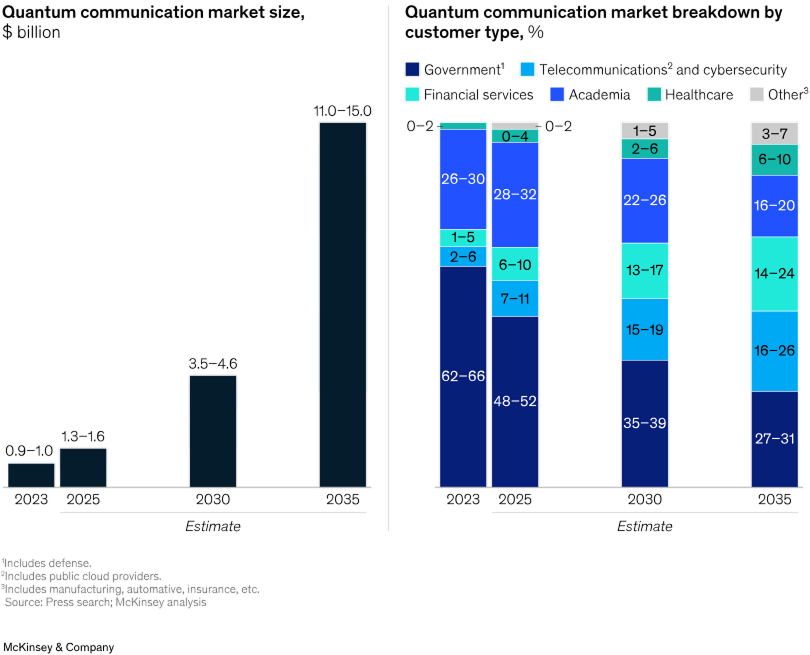
\includegraphics[width=0.9\linewidth]{qt351.png}
	\caption{Quantum Communication market size projectionby 2035}
	\label{fig:enter-label}
\end{figure}